% Dokumentenklasse
\documentclass{article}

% Pakete
\usepackage{tex/pakete}
\usepackage{tex/macros}

% Einstellen der Pakete
\graphicspath{{figs/}}
\addbibresource{refs.bib}
\titleformat{\section}
  {\normalfont\LARGE\bfseries}{\thesection.}{.3em}{}
\titlespacing*{\section}{0pt}{3.5ex plus 1ex minus .2ex}{2.3ex plus .2ex}
\titleformat{\subsection}
  {\normalfont\Large\bfseries}{\thesubsection.}{.3em}{}
\titlespacing*{\subsection}{0pt}{3.5ex plus 1ex minus .2ex}{2.3ex plus .2ex}
\titleformat{\subsubsection}
  {\normalfont\large\bfseries}{\thesubsubsection.}{.3em}{}
\titlespacing*{\subsubsection}{0pt}{3.5ex plus 1ex minus .2ex}{2.3ex plus .2ex}

\sisetup{output-decimal-marker = {,}}

%\numberwithin{equation}{section}
%\counterwithin{figure}{section}

\pagestyle{fancy}
%\fancyhf{}
\lhead{P428 Röntgenstrahlung und Materialanalyse}
\rhead{Gabriel Remiszewski und Christian Fischer}

% Titelblatt
\title{\textbf{Versuchsbericht} \\ \Large{\textbf{P428 Röntgenstrahlung und Materialanalyse}}}
\date{durchgeführt am 15/16.11.2023}
\author{Gabriel Remiszewski und Christian Fischer}

%========================================================================
\begin{document}

\begin{titlepage}
\maketitle
\thispagestyle{empty}
\end{titlepage}
\newpage
\tableofcontents
\thispagestyle{empty}
\newpage

% "Einleitung"
\section{Einleitung}\label{sec:einleitung}
\pagenumbering{arabic}
\cite{skript}

% "Versuchsabschnitte"
\section{Laue-Aufnahme}\label{sec:laue}
In diesem Versuchsteil wird die Symmetrie und Gitterstruktur eines NaCl-Kristalls mithilfe des Laue-Verfahrens untersucht. Dabei wird der zu
untersuchende Kristall mit Röntgenstrahlung bestrahlt. Hinter dem Kristall ist ein Röntgenfilm platziert, auf dem die durch den Kristall laufende
Röntgenstrahlung nachgewiesen werden kann. Mithilfe des auf dem Röntgenfilm entstehenden Musters können dann einige Eigenschaften des verwendeten
Kristalls untersucht werden.
\subsection{Aufbau}\label{subsec:laue_aufbau}
Zur Durchführung dieses Versuchsteils wird der zu Verfügung stehende NaCl-Kristall verwendet. Die Röntgenstrahlung wird mit einer Molybdän-Röntgenröhre
erzeugt. Der Versuchsaufbau zur Laue-Aufnahme ist in \cref{fig:aufbau_laue} dargestellt.
\begin{figure}[H]
	\centering
	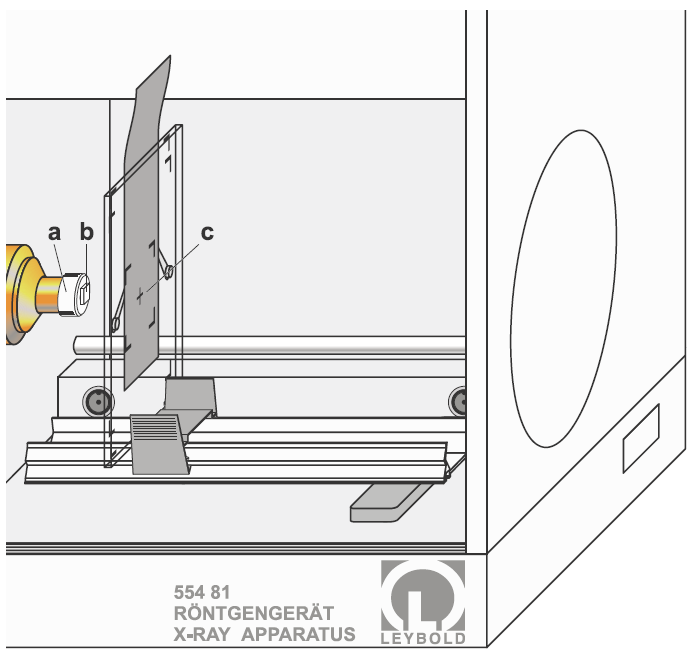
\includegraphics[width=0.6\linewidth]{../figs/aufbau_laue.png}
	\caption{Versuchsaufbau der Laue-Aufnahme zur Untersuchung eines NaCl-Kristalls:
    a - Lochblende, b - NaCl-Kristall, c - Röntgenfilm  \cite{laue_handblatt}.}
	\label{fig:aufbau_laue}
\end{figure} Zunächst wird die Molybdän-Röntgenröhre zur Erzeugung der benötigten Röntgenstrahlung eingesetzt. Aus dem Vollschutzröntgengerät werden Targethalter
und Sensorarm entfernt, sodass eine Experimentierschiene mittig vor die Kollimatoraufnahme platziert werden kann. In die Kollimatoraufnahme wird der Kollimator
mit \SI{1}{\milli \meter} Spaltbreite eingesetzt. Der verwendete NaCl-Kristall ist bereits auf einer Lochblende befestigt, welche deshalb sofort auf den Kollimator aufgesetzt
werden kann. Für die Laue-Aufnahme wird ein \textit{AGFA Dentus M2 Comfort} Röntgenfilm verwendet, welcher möglichst mittig auf der markierten Fläche
des Filmhalters festgeklemmt wird. Dabei muss darauf geachtet werden, dass der Film möglichst plan über seine gesamte Fläche aufliegt. Außerdem muss die weiße Seite des
Films zur Röntgenröhre zeigen. Anschließend wird der Filmhalter auf der Experimentierschiene platziert und verschoben, sodass zwischen NaCl-Kristall und Film ein Abstand von \SI{15(2)}{\milli \meter} (hier gibt es eine relativ große Unsicherheit,
da die Einstellung nicht allzu exakt vorgenommen werden konnte) eingestellt wird.\par
An dem Vollschutzröntgengerät wird eine Röhrenhochspannung von $U = \SI{35,0}{\kilo \volt}$ und ein Emissionsstrom von $I = \SI{1,0}{\milli \ampere}$ eingestellt.
Die Winkeländerung des Goniometers wird auf $\Delta \beta = \SI{0,0}{\degree}$ eingestellt. Schließlich wird die Messzeit auf $\Delta t = \SI{1800}{\second}$ eingestellt.
\subsection{Messung}\label{subsec:laue_messung}
Mithilfe des Tasters \texttt{SCAN} auf dem Vollschutzröntgengerät kann die Belichtungsuhr gestartet werden. Nach Ablauf der Belichtungszeit wird der Röntgenfilm entnommen
und kann dann mithilfe der beiliegenden Entwicklungsausrüstung entwickelt werden. Der lichtdicht in eine Kunststoffhülle eingeschweißte Röntgenfilm kann nun
in einer Tageslicht-Entwicklerdose entwickelt werden. Das Öffnen der Kunststoffhülle und Einlegen des Röntgenfilms in die Tageslicht-Entwicklerdose erfolgt
in einem lichtdichten Wechselsack. Die gesamte Entwicklung wird nun exakt wie in der beigelegten Gebrauchsanweisung durchgeführt, welche in \cite{film_anleitung} hinterlegt ist.\par
Der fertig entwickelte Röntgenfilm kann dann eingescannt (schwarz-weiß) werden, was zur weiteren Auswertung dient. Die beiden eingescannten Seiten des Röntgenfilms sind
in \cref{fig:eingescannter_film} dargestellt. Es ist zu erkennen, dass sich auf dem fertig entwickelten Röntgenfilm ein relativ großer Fleck befindet, dessen Auftreten später
diskutiert wird. Allerdings wird für die Auswertung nur die Seite des Röntgenfilms verwendet, bei der die Reflexe (kleine schwarze Flecken) trotz des Flecks bestmöglich erkannt werden können (siehe \cref{fig:eingescannter_film}, links).
\begin{figure}[H]
    \centering
    \begin{subfigure}{0.45\textwidth}
        \centering
        \includegraphics[width=\linewidth]{../figs/hochauflösend_1_edit}
        \caption{}\label{fig:links}
    \end{subfigure}
    \begin{subfigure}{0.45\textwidth}
        \centering
        \includegraphics[width=\linewidth]{../figs/hochauflösend_2_edit}
        \caption{}
    \end{subfigure}
    \caption{Entwickelter Röntgenfilm zur weiteren Auswertung.}\label{fig:eingescannter_film}
\end{figure} Abschließend werden noch die Abmessungen des Röntgenfilms bestimmt, da dies für die Auswertung benötigt wird. Der Röntgenfilm ist \SI{57(1)}{\milli \meter} breit und \SI{76(1)}{\milli \meter} hoch.
\subsection{Auswertung}\label{subsec:laue_auswertung}
%\begin{table}[H]
%    \centering
%    \caption{Miller-Indizes}
%    \begin{tabular}{c|c|c|c|c|c|c|c}
%        Punkt & $x_{\mathrm{P}}'$ / p & $y_{\mathrm{P}}'$ / p & $x_{\mathrm{P}}$ / p & $y_{\mathrm{P}}$ / p & $z_{\mathrm{Q}}$ / p & $\Delta z_{\mathrm{Q}}$ / p & $(h,k,l)$ \\
%        \hline
%        A01 & 1289 & 1665 & -273 & -184 & 106 & 18 & $(\bar{5}\bar{3}2)$ \\
%        A02 & 1364 & 1660 & -198 & -189 &  75 & 14 & $(\bar{5}\bar{5}2)$ \\
%        A03 & 1360 & 1589 & -202 & -260 & 106 & 18 & $(\bar{3}\bar{5}2)$ \\
%        A04 & 1739 & 1538 &  177 & -311 & 123 & 20 & $(3\bar{5}2)$ \\
%        A05 & 1762 & 1623 &  200 & -226 &  90 & 16 & $(5\bar{5}2)$ \\
%        A06 & 1862 & 1623 &  300 & -226 & 134 & 21 & $(5\bar{3}2)$ \\
%        A07 & 1875 & 2058 &  313 &  209 & 134 & 21 & $(532)$ \\
%        A08 & 1776 & 2072 &  214 &  223 &  94 & 17 & $(552)$ \\
%        A09 & 1762 & 2158 &  200 &  309 & 129 & 21 & $(352)$ \\
%        A10 & 1363 & 2121 & -199 &  272 & 110 & 19 & $(\bar{3}52)$ \\
%        A11 & 1363 & 2030 & -199 &  181 &  73 & 14 & $(\bar{5}52)$ \\
%        A12 & 1283 & 2018 & -279 &  169 & 104 & 18 & $(\bar{5}32)$ \\
%        B01 & 1507 & 1638 &  -55 & -211 &  49 & 11 & $(\bar{1}\bar{4}1)$ \\
%        B02 & 1579 & 1623 &   17 & -226 &  53 & 11 & $(1\bar{4}1)$ \\
%        B03 & 1807 & 1793 &  245 &  -56 &  64 & 13 & $(4\bar{1}1)$ \\
%        B04 & 1810 & 1908 &  248 &   59 &  66 & 13 & $(411)$ \\
%        B05 & 1597 & 2086 &   35 &  237 &  59 & 12 & $(141)$ \\
%        B06 & 1507 & 2075 &  -55 &  226 &  55 & 12 & $(\bar{1}41)$ \\
%        B07 & 1360 & 1884 & -202 &   35 &  44 & 10 & $(\bar{4}11)$ \\
%        B08 & 1362 & 1803 & -200 &  -46 &  44 & 10 & $(\bar{4}\bar{4}1)$ \\
%        C01 & 1414 & 1482 & -148 & -367 & 147 & 23 & $(\bar{2}\bar{5}2)$ \\
%        C02 & 1535 & 1416 &  -27 & -433 & 172 & 25 & $(0\bar{5}2)$ \\
%        C03 & 1672 & 1450 &  110 & -399 & 159 & 24 & $(2\bar{5}2)$ \\
%        C04 & 1974 & 1695 &  412 & -154 & 176 & 26 & $(\bar{5}\bar{2}2)$ \\
%        C05 & 2039 & 1835 &  477 &  -14 & 203 & 28 & $(\bar{5}02)$ \\
%        C06 & 1983 & 1985 &  421 &  136 & 178 & 26 & $(522)$ \\
%        C07 & 1689 & 2248 &  127 &  399 & 162 & 24 & $(252)$ \\
%        C08 & 1548 & 2286 &  -14 &  437 & 175 & 26 & $(052)$ \\
%        C09 & 1422 & 2222 & -140 &  373 & 148 & 23 & $(\bar{2}52)$ \\
%        C10 & 1200 & 1958 & -362 &  109 & 135 & 22 & $(\bar{5}22)$ \\
%        C11 & 1161 & 1843 & -401 &   -6 & 150 & 23 & $(\bar{5}02)$ \\
%        C12 & 1205 & 1730 & -357 & -119 & 134 & 21 & $(\bar{5}\bar{2}2)$ \\
%        D01 & 1236 & 1543 & -326 & -306 & 181 & 26 & $(\bar{4}\bar{4}2)$ \\
%        D02 & 1891 & 1478 &  329 & -371 & 216 & 29 & $(4\bar{4}2)$ \\
%        D03 & 1913 & 2205 &  351 &  356 & 219 & 29 & $(442)$ \\
%        D04 & 1236 & 2152 & -326 &  303 & 180 & 26 & $(\bar{4}42)$ \\
%        E01 & 1025 & 1585 & -357 & -264 & 179 & 26 & $(\bar{4}\bar{2}2)$ \\
%        E02 & 1262 & 1302 & -300 & -547 & 315 & 36 & $(\bar{2}\bar{4}2)$ \\
%        E03 & 1830 & 1239 &  268 & -610 & 350 & 40 & $(2\bar{4}2)$ \\
%        E04 & 2175 & 1516 &  613 & -333 & 380 & 40 & $(4\bar{2}2)$ \\
%        E05 & 2204 & 2169 &  642 &  320 & 390 & 40 & $(422)$ \\
%        E06 & 1859 & 2462 &  297 &  613 & 360 & 40 & $(242)$ \\
%        E07 & 1262 & 2402 & -300 &  553 & 320 & 40 & $(\bar{2}42)$ \\
%        E08 & 1017 & 2104 & -545 &  255 & 300 & 40 & $(\bar{4}22)$ \\
%        F01 &  850 & 1390 & -712 & -459 & 500 & 50 & $(\bar{3}\bar{2}2)$ \\
%        F02 & 1057 & 1147 & -505 & -702 & 520 & 50 & $(\bar{2}\bar{3}2)$ \\
%        F03 & 2069 & 1016 &  507 & -833 & 620 & 50 & $(2\bar{3}2)$ \\
%        F04 & 2388 & 1260 &  826 & -589 & 650 & 50 & $(3\bar{2}2)$ \\
%        F05 & 2430 & 2431 &  868 &  582 & 680 & 50 & $(322)$ \\
%        F06 & 2115 & 2684 &  553 &  835 & 640 & 50 & $(232)$ \\
%        F07 & 1048 & 2583 & -514 &  734 & 540 & 50 & $(\bar{2}32)$ \\
%        F08 &  834 & 2309 & -728 &  460 & 520 & 50 & $(\bar{3}22)$                
%    \end{tabular}\label{tab:miller}
%\end{table}\newpage
Bevor der fertig entwickelte Röntgenfilm systematisch analysiert wird, werden einige Beobachtungen diskutiert, welche in \cref{fig:eingescannter_film} festgestellt werden können.
Zunächst ist auf dem Röntgenfilm ein großer Fleck zu erkennen. Auf der einen Seite des Röntgenfilms ist dieser Fleck sogar so intensiv, dass einige der Reflexe nicht mehr erkannt werden können.
Glücklicherweise ist dieser Fleck auf der anderen Seite des Röntgenfilms etwas weniger intensiv, sodass hier alle wichtigen Reflexe erkannt werden können. Das
Zustandekommen des Flecks lässt sich nicht eindeutig begründen, allerdings besteht die Vermutung, dass der Röntgenfilm bei der Entwicklung nicht optimal in der
Tageslicht-Entwicklerdose befestigt war, sodass die Entwickler- und Fixier-Lösung (siehe \cite{film_anleitung}) nicht den gesamten Röntgenfilm getroffen hat. Eventuell wurde
bei der Entwicklung auch das Schwenken der Tageslicht-Entwicklerdose zu sanft gehandhabt, weshalb nicht der gesamte Film gleichmäßig von der Entwickler- und Fixier-Lösung
getroffen wurde. Ein weiterer möglicher Grund für das Entstehen des Flecks ist, dass etwas Licht im Experimentierraum auf den Röntgenfilm getroffen ist, bevor dieser
fertig entwickelt war. Dies ist jedoch unwahrscheinlich, da das Entfernen des Röntgenfilms aus der Kunststoffhülle und das Einbringen in die Tageslicht-Entwicklerdose
mit größter Vorsicht und nach Anleitung vorgenommen wurde.\par
Außerdem ist in \cref{fig:eingescannter_film} zu erkennen, dass viele der Reflexe leicht verschmiert sind. Die Reflexe sind die beobachteten dunklen Stellen, welche durch das
Auftreffen von Röntgenstrahlung auf den Röntgenfilm verursacht werden. Auch für das Verschmieren der Reflexe können die Ursachen vielfältig sein, wie z.B.
dass der Abstand zwischen Röntgenfilm und NaCl-Kristall nicht optimal eingestellt war. Hier war eine exakte Einstellung schwierig, da der verwendete Längen-Maßstab
nicht passend zwischen Röntgenfilm und NaCl-Kristall gehalten werden konnte. Um diese Fehlerquelle bei der Auswertung zu berücksichtigen, wird die Unsicherheit
für den gemessenen Abstand $L = \SI{15}{\milli \meter}$ grob auf $\Delta L = \SI{2}{\milli \meter}$ abgeschätzt. Außerdem ist es möglich, dass der untersuchte NaCl-Kristall mittlerweile einige Verunreinigungen
aufweist, wobei dies nur eine Vermutung ist, die nicht anderweitig nachgewiesen werden kann.\par
Zudem fällt auf, dass das entstandene Bild auf dem Röntgenfilm leicht gewölbt ist. Der größte Beitrag dafür kann darauf zurückgeführt werden, dass der Röntgenfilm
nicht über seine gesamte Fläche plan auf der markierten Fläche des Filmhalters auflag. Schließlich ist auch zu erkennen, dass die Symmetrieachsen des entstandenen Reflex-Musters
nicht mit den Spiegelachsen des Röntgenfilms zusammenfallen. Diese Drehung kommt wahrscheinlich dadurch zustande, dass die Lochblende mit dem aufgesetzten NaCl-Kristall nicht so gedreht wurde,
dass die Außenkanten des Kristalls möglichst genau horizontal bzw. vertikal verlaufen. Beide diese Fehler hätten durch eine präzisere Justierung leicht vermieden werden können. Jedoch spielt dies für die
weitere Auswertung nur eine untergeordnete Rolle, da sich die Reflexe dennoch gut auswerten lassen.\\ \par
Das Ziel ist nun die Zuordnung der für die Streuung verursachenden Netzebenenschar zu einem auf dem Röntgenfilm beobachteten Reflex. Ein Großteil der Röntgenstrahlung
durchläuft den NaCl-Kristall ohne Streuung, wodurch der mittige große schwarze Fleck auf dem Röntgenfilm verursacht wird. Zudem wird ein Teil der Röntgenstrahlung
an den Gitterebenen des NaCl-Kristalls gestreut. In eine bestimmte Richtung kommt es nur dann zu konstruktiver Interferenz der an einer Netzebenenschar reflektierten
Röntgenstrahlung, wenn die Laue-Bedingung erfüllt ist, also die Änderung des Wellenvektors einem reziproken Gittervektor entspricht. Dies führt dann zu einem
Reflex auf dem Röntgenfilm. Weitere Informationen zu der Laue-Bedingung sind in \cite{kristalle} zu finden.\par
Die Symmetrie des Musters in \cref{fig:eingescannter_film} lässt sich auf die kubische Symmetrie der Elementarzellen des NaCl-Kristalls zurückführen (siehe \cref{fig:elementarzelle_nacl}).
\begin{figure}[H]
	\centering
	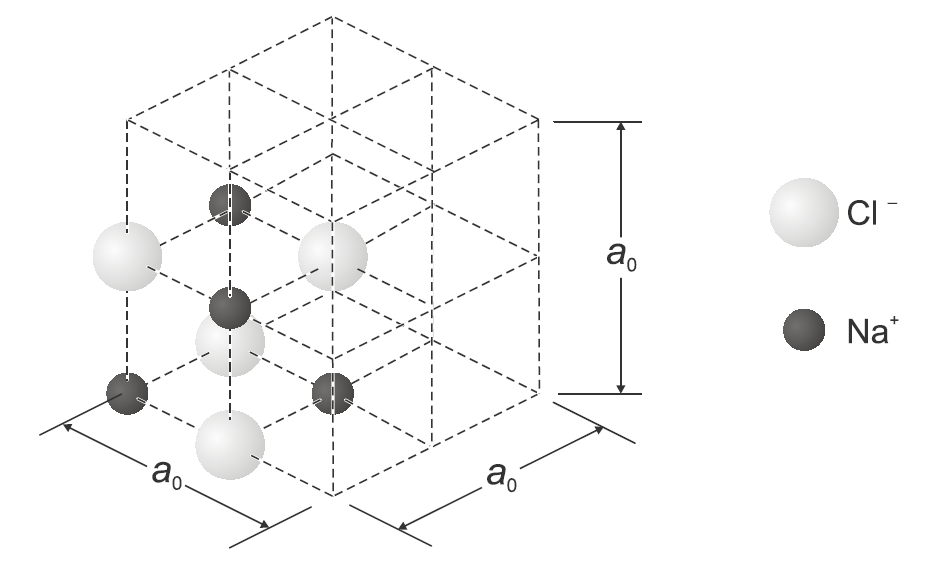
\includegraphics[width=0.6\linewidth]{../figs/elementarzelle_nacl.png}
	\caption{Elementarzelle des NaCl-Kristalls \cite{laue_handblatt}.}
	\label{fig:elementarzelle_nacl}
\end{figure}
Um nun einem auf dem Röntgenfilm beobachteten Reflex die für die Streuung verantwortliche Netzebenenschar zuzuordnen, wird das Koordinatensystem wie in \cref{fig:skizze}
gewählt. Eine Netzebenenschar setzt sich aus zueinander parallel liegenden Netzebenen im Kristall zusammen, die den Netzebenenabstand $d_{\mathrm{hkl}}$ voneinander haben.
Die Orientierung einer solchen Netzebenenschar wird durch die Millerschen Indizes $(hkl)$ beschrieben, da der Vektor $(h,k,l)$, welcher durch die
Millerschen Indizes gebildet wird, als Normalenvektor senkrecht auf der Netzebenenschar steht. 
\begin{figure}[H]
	\centering
	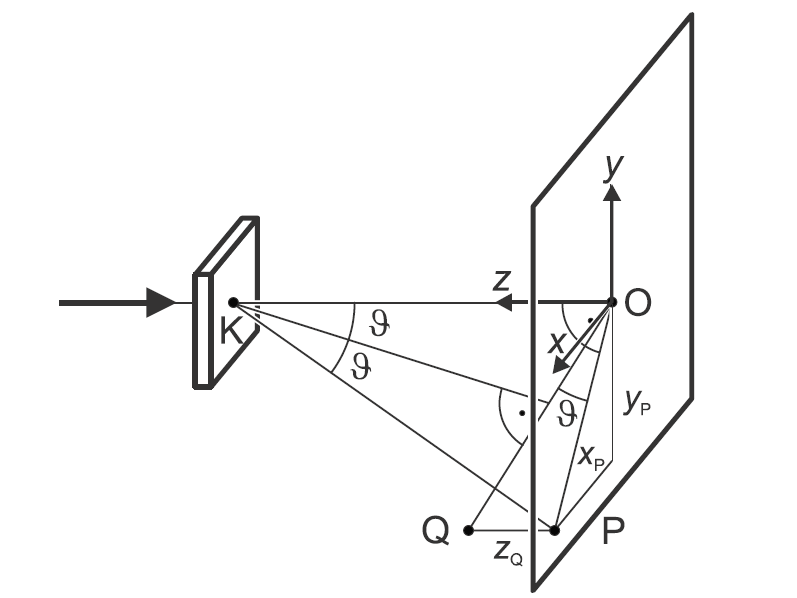
\includegraphics[width=0.6\linewidth]{../figs/skizze.png}
	\caption{Geometrische Beschreibung eines im Punk $K$ des Kristalls gebeugten Röntgenstrahls, der die Filmebene im Punkt $P$ durchdringt \cite{laue_handblatt}.}
	\label{fig:skizze}
\end{figure} In \cref{fig:skizze} wird das Koordinatensystem so gewählt, dass sein Ursprung dem Aufpunkt des einfallenden Röntgenstrahls auf dem
Röntgenfilm entspricht. Der Röntgenfilm steht senkrecht zum Strahl, d.h. er liegt in der $x$-$y$-Ebene. Der Röntgenstrahl durchdringt den flachen Kristall im Punkt $K$.
Der ungebeugte Anteil der Röntgenstrahlung trifft im Ursprung auf den Röntgenfilm und der Anteil der Röntgenstrahlung, der in $K$ gestreut wird und die Laue-Bedingung
erfüllt, verlässt den Kristall unter dem Winkel $2\theta$ zur Primärstrahlung und trifft im Punkt $P = (x_{\mathrm{P}}, y_{\mathrm{P}}, 0)$ auf den Röntgenfilm. Hier ist
$\theta$ der Glanzwinkel. Der Abstand zwischen Kristall und Röntgenfilm sei $L$. Die Winkelhalbierende des Winkels $2\theta$ gibt die Richtung der Netzebenenschar $(hkl)$ an,
die den Reflex verursacht. Es wird ein weiterer Punkt $Q = (x_{\mathrm{P}}, y_{\mathrm{P}}, z_{\mathrm{Q}})$ zur geometrischen Konstruktion eingeführt.
In \cite{laue_handblatt} wird gezeigt, dass
\begin{equation}\label{eq:koordinate}
    z_{\mathrm{Q}} = \sqrt{x_{\mathrm{P}}^2 + y_{\mathrm{P}}^2 + L^2} - L
\end{equation} gilt. Die Millerschen Indizes erfüllen dann die Bedingung
\begin{equation}\label{eq:indizes}
    h:k:l = x_{\mathrm{P}}:y_{\mathrm{P}}:z_{\mathrm{Q}} . 
\end{equation} Somit kann \cref{eq:indizes} zur Bestimmung der Millerschen Indizes verwendet werden. Diese sind daher kleinste ganzzahlige Zahlentripel.
Aus ihnen können alle Parameter der den Reflex verursachenden Beugung berechnet werden. In \cite{laue_handblatt} wird außerdem gezeigt, dass für Kristalle mit
NaCl-Struktur die Amplituden der von den Elementarzellen ausgehenden Wellen nur dann von Null verschieden sind, wenn alle Indizes $h$, $k$ und $l$ gerade und oder alle ungerade sind.
Dies wird später für die Bestimmung der Millerschen Indizes wichtig.\\ \par
Um den eingescannten Röntgenfilm auszuwerten, wird das Bildbearbeitungs-Programm \texttt{paint.net} verwendet. Zunächst wird das linke Bild des Röntgenfilms aus
\cref{fig:eingescannter_film} so gedreht, dass die Symmetrieachsen des Musters bestmöglich mit der Wahl der Koordinatensystems zusammenpassen. Dann wird an jeden ausreichend
erkennbaren Reflex eine Ellipse angepasst, sodass später die Koordinaten $x_{\mathrm{P}}$ und $y_{\mathrm{P}}$ eines Reflexes als Mittelpunkt einer solchen Ellipse identifiziert
werden können. Die Anpassung kann aufgrund der leichten Verschmierung der Reflexe nur mit einer gewissen Genauigkeit zugeordnet werden, was später in
der Ableseunsicherheit für die Mittelpunkte berücksichtigt wird. Für die Ellipsen werden unterschiedliche Farben gewählt, sodass das Muster der Reflexe
besser erkannt werden kann. Die Wahl der Farben hat hier keine physikalische Bedeutung und ist willkürlich. In dem Programm können dann die Pixelkoordinaten
des Ursprungs und der Mittelpunkte der an die Reflexe angepassten Ellipsen abgelesen werden. Die Darstellung des Röntgenfilms wird so gewählt, dass die in der
Informatik übliche Konvention für Pixelkoordinaten ($x$-Achse nach rechts, $y$-Achse nach unten) mit dem in \cref{fig:skizze} gewählten Koordinatensystem übereinstimmt.
Die fertig erstellte Grafik ist in \cref{fig:reflexe} zu sehen. Für das Ablesen der Pixelkoordinaten wird eine Unsicherheit von \SI{10}{\px} gewählt, da die Ellipsen
bei fast allen Reflexen mit der gleichen Genauigkeit angepasst werden konnten und somit für das Ablesen der Mittelpunkte die gleiche Unsicherheit besteht.
\begin{figure}[H]
	\centering
	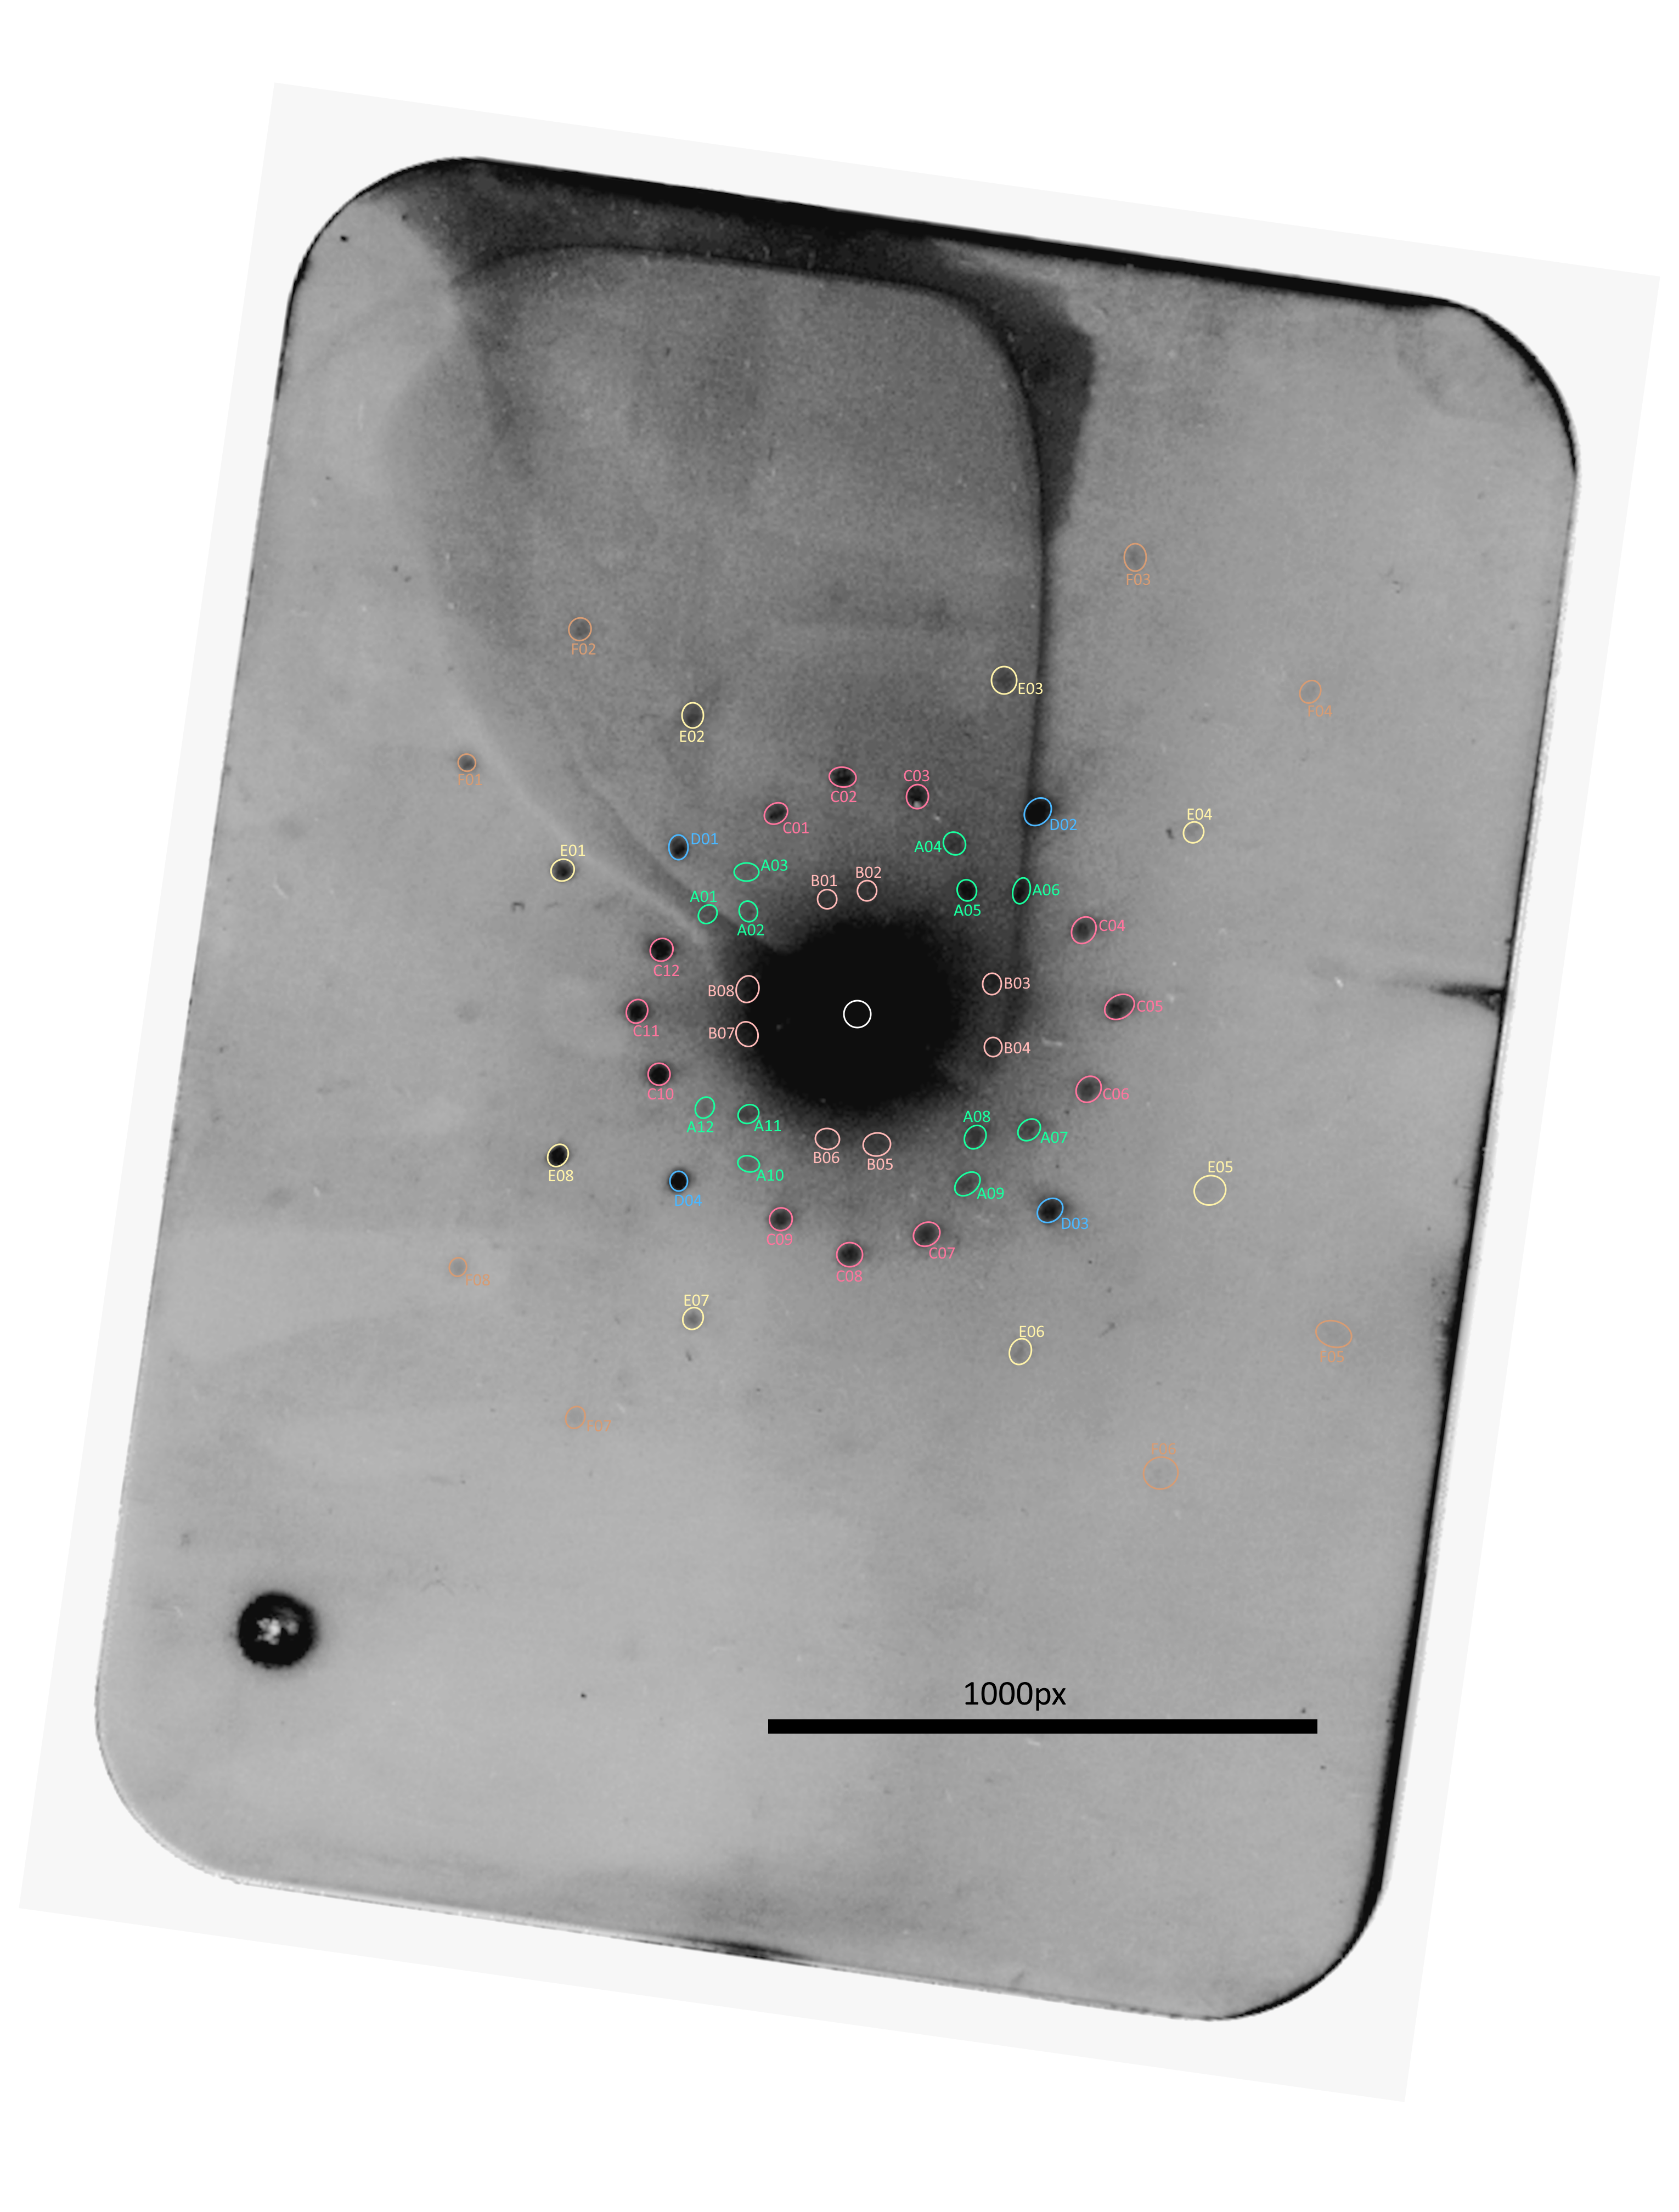
\includegraphics[width=0.9\linewidth]{../figs/reflexe.png}
	\caption{Graphische Bearbeitung des Röntgenfilms zur Auswertung der Reflexe und Bestimmung der Millerschen Indizes.}
	\label{fig:reflexe}
\end{figure} Die Pixelkoordinaten des Ursprungs werden zu $x_{\mathrm{O}}' = \SI{1562(10)}{\px}$ und $y_{\mathrm{O}}' = \SI{1849(10)}{\px}$ abgelesen. Analog werden
die Pixelkoordinaten der Reflexe $x_{\mathrm{P}}'$ und $y_{\mathrm{P}}'$ abgelesen. Die Pixelkoordinaten für das gewählte Koordinatensystem ergeben sich dann durch
\begin{equation*}
    x_{\mathrm{P}} = x_{\mathrm{P}}' - x_{\mathrm{O}}' , \quad y_{\mathrm{P}} = y_{\mathrm{P}}' - y_{\mathrm{O}}'
\end{equation*} mit den Unsicherheiten
\begin{equation*}
    \Delta x_{\mathrm{P}} = \sqrt{(\Delta x_{\mathrm{P}}')^2 + (\Delta x_{\mathrm{O}}')^2} , \quad \Delta y_{\mathrm{P}} = \sqrt{(\Delta y_{\mathrm{P}}')^2 + (\Delta y_{\mathrm{O}}')^2} .
\end{equation*} Nun kann die Koordinate $z_{\mathrm{Q}}$ in px analog zu \cref{eq:koordinate} gemäß
\begin{equation*}
    z_{\mathrm{Q}} = \sqrt{x_{\mathrm{P}}^2 + y_{\mathrm{P}}^2 + (c L)^2} - c L
\end{equation*} berechnet werden, wobei mit dem Faktor $c$ die Länge $L$ von \unit{\milli \meter} in px umgerechnet wird. Die (quadrierte) Unsicherheit ist durch
\begin{align*}
    (\Delta z_{\mathrm{Q}})^2 &= \left(\frac{x_{\mathrm{P}} \Delta x_{\mathrm{P}}}{\sqrt{x_{\mathrm{P}}^2 + y_{\mathrm{P}}^2 + (c L)^2}}\right)^2
                                +\left(\frac{y_{\mathrm{P}} \Delta y_{\mathrm{P}}}{\sqrt{x_{\mathrm{P}}^2 + y_{\mathrm{P}}^2 + (c L)^2}}\right)^2 \\
                              &\quad+ \left(\left[\frac{c^2 L}{\sqrt{x_{\mathrm{P}}^2 + y_{\mathrm{P}}^2 + (c L)^2}} - c\right] \Delta L\right)^2
                                +\left(\left[\frac{c L^2}{\sqrt{x_{\mathrm{P}}^2 + y_{\mathrm{P}}^2 + (c L)^2}} - L\right] \Delta c\right)^2
\end{align*} gegeben. Der Umrechnungsfaktor $c$ wird als fehlergewichteter Mittelwert aus $c_1$ und $c_2$ gemäß
\begin{equation*}
    c = \frac{\frac{c_1}{(\Delta c_1)^2} + \frac{c_2}{(\Delta c_2)^2}}{\frac{1}{(\Delta c_1)^2} + \frac{1}{(\Delta c_2)^2}} , \quad
    \Delta c = \frac{1}{\sqrt{\frac{1}{(\Delta c_1)^2} + \frac{1}{(\Delta c_2)^2}}}
\end{equation*} berechnet, wobei $c_1$ und $c_2$ die entsprechenden Umrechnungsfaktoren für Breite und Höhe des Röntgenfilms von \unit{\milli \meter} in px sind.
Beide dieser Umrechnungsfaktoren berechnen sich gemäß
\begin{equation*}
    c_i = \frac{l_{\mathrm{px}}}{l_{\unit{\milli \meter}}}, \quad \Delta c_i = \sqrt{\left(\frac{\Delta l_{\mathrm{px}}}{l_{\unit{\milli \meter}}}\right)^2 + \left(\frac{l_{\mathrm{px}}}{l_{\unit{\milli \meter}}^2}\Delta l_{\unit{\milli \meter}}\right)^2} \quad (i = 1,2),
\end{equation*} wobei die Länge $l$ entweder die Breite oder Höhe des Röntgenfilms (in px oder \unit{\milli \meter}) beschreibt. Für die Breite
des Röntgenfilms wurde \SI{57(1)}{\milli \meter} (bzw. \SI{2382}{\px}) und für die Höhe \SI{76(1)}{\milli \meter} (bzw. \SI{3182}{\px}) gemessen (bzw. abgelesen).
Es ergibt sich
\begin{equation*}
    c_1 = \SI{41,8(8)}{\frac{\px}{\milli \meter}} , \quad c_2 = \SI{41,9(6)}{\frac{\px}{\milli \meter}}
\end{equation*} und damit
\begin{equation*}
    c = \SI{42,8(5)}{\frac{\px}{\milli \meter}} .
\end{equation*} Nun kann $z_{\mathrm{Q}}$ in px berechnet werden. Die Koordinaten $x_{\mathrm{P}}$, $y_{\mathrm{P}}$ und $z_{\mathrm{Q}}$ (inklusive $\Delta z_{\mathrm{Q}}$) sind in \cref{tab:miller2} eingetragen.
Wie schon zuvor erwähnt, wird für $x_{\mathrm{P}}$ und $y_{\mathrm{P}}$ eine Unsicherheit von \SI{10}{\px} gewählt. Somit können nun die Millerschen Indizes der
für die Reflexe verantwortlichen Netzebenenscharen nach \cref{eq:indizes} bestimmt werden.\par
Hierzu wird wie folgt vorgegangen: Zuerst wird willkürlich $l = 1$ gesetzt. Dann
sind die Indizes $h$ und $k$ durch die Verhältnisse $h = \frac{x_{\mathrm{P}}}{z_{\mathrm{Q}}}$ und $k = \frac{y_{\mathrm{P}}}{z_{\mathrm{Q}}}$ eindeutig bestimmt. Anschließend
werden die Indizes $(hkl)$ mit einem ganzzahligen Faktor multipliziert, sodass die Indizes $h$ und $k$ möglichst eine ganze Zahl annehmen und die Indizes $(hkl)$ entweder
alle gerade oder alle ungerade sind (wie bereits zuvor erläutert). Hierbei tritt natürlch häufig die Schwierigkeit auf, dass durch das Multiplizieren mit einem ganzzahligen Faktor
die Indizes $h$ und $k$ nicht exakt eine ganze Zahl annehmen, sondern meistens nur in der Umgebung einer naheliegenden ganzen Zahl liegen. Dies ist jedoch meist kein Problem bei
der Zuordnung der Millerschen Indizes, da $x_{\mathrm{P}}$, $y_{\mathrm{P}}$ und $z_{\mathrm{Q}}$ allesamt eine Unsicherheit besitzen. In den meisten Fällen ist jedoch klar
ersichtlich, welche ganze Zahl am nächsten liegt. Es werden stets die Millerschen Indizes gemeinsam bestimmt, die aus Symmetriegründen sich nur durch Vorzeichen und Permutation voneinander
unterscheiden. Hier können dann leicht Ausreißer erkannt und entsprechend korrigiert werden, sodass die verschiedenen Paare an Millerschen Indizes mit den Symmetrieeigenschaften
des NaCl-Kristalls übereinstimmen. Alle bestimmten Millerschen Indizes sind ebenfalls in \cref{tab:miller2} eingetragen.\newpage
\begin{table}[H]
    \centering
    \caption{Miller-Indizes}
    \begin{tabular}{c|c|c|c|c|c|c|c}
        Punkt & $x_{\mathrm{P}}'$ / px & $y_{\mathrm{P}}'$ / px & $x_{\mathrm{P}}$ / px & $y_{\mathrm{P}}$ / px & $z_{\mathrm{Q}}$ / px & $\Delta z_{\mathrm{Q}}$ / px & $(hkl)$ \\
        \hline
        A01 & $1289$ & $1665$ & $-273$ & $-184$ & $ 81$ & $13$ & $(\bar{6}\bar{4}2)$ \\
        A02 & $1364$ & $1660$ & $-198$ & $-189$ & $ 57$ & $10$ & $(\bar{3}\bar{3}1)$ \\
        A03 & $1360$ & $1589$ & $-202$ & $-260$ & $ 81$ & $13$ & $(\bar{4}\bar{6}2)$ \\
        A04 & $1739$ & $1538$ & $ 177$ & $-311$ & $ 95$ & $14$ & $(4\bar{6}2)$ \\
        A05 & $1762$ & $1623$ & $ 200$ & $-226$ & $ 69$ & $11$ & $(3\bar{3}1)$ \\
        A06 & $1862$ & $1623$ & $ 300$ & $-226$ & $104$ & $15$ & $(6\bar{4}2)$ \\
        A07 & $1875$ & $2058$ & $ 313$ & $ 209$ & $104$ & $15$ & $(642)$ \\
        A08 & $1776$ & $2072$ & $ 214$ & $ 223$ & $ 72$ & $12$ & $(331)$ \\
        A09 & $1762$ & $2158$ & $ 200$ & $ 309$ & $100$ & $14$ & $(462)$ \\
        A10 & $1363$ & $2121$ & $-199$ & $ 272$ & $ 85$ & $13$ & $(\bar{4}62)$ \\
        A11 & $1363$ & $2030$ & $-199$ & $ 181$ & $ 55$ & $10$ & $(\bar{3}31)$ \\
        A12 & $1283$ & $2018$ & $-279$ & $ 169$ & $ 80$ & $13$ & $(\bar{6}42)$ \\
        B01 & $1507$ & $1638$ & $ -55$ & $-211$ & $ 37$ & $ 7$ & $(\bar{2}(\bar{12})2)$ \\
        B02 & $1579$ & $1623$ & $  17$ & $-226$ & $ 40$ & $ 7$ & $(2(\bar{12})2)$ \\
        B03 & $1807$ & $1793$ & $ 245$ & $ -56$ & $ 48$ & $10$ & $((12)\bar{2}2)$ \\
        B04 & $1810$ & $1908$ & $ 248$ & $  59$ & $ 50$ & $10$ & $((12)22)$ \\
        B05 & $1597$ & $2086$ & $  35$ & $ 237$ & $ 44$ & $ 8$ & $(2(12)2)$ \\
        B06 & $1507$ & $2075$ & $ -55$ & $ 226$ & $ 42$ & $ 8$ & $(\bar{2}(12)2)$ \\
        B07 & $1360$ & $1884$ & $-202$ & $  35$ & $ 33$ & $ 8$ & $((\bar{12})22)$ \\
        B08 & $1362$ & $1803$ & $-200$ & $ -46$ & $ 33$ & $ 8$ & $((\bar{12})\bar{2}2)$ \\
        C01 & $1414$ & $1482$ & $-148$ & $-367$ & $114$ & $16$ & $(\bar{1}\bar{3}1)$ \\
        C02 & $1535$ & $1416$ & $ -27$ & $-433$ & $135$ & $17$ & $(0\bar{3}1)$ \\
        C03 & $1672$ & $1450$ & $ 110$ & $-399$ & $124$ & $16$ & $(1\bar{3}1)$ \\
        C04 & $1974$ & $1695$ & $ 412$ & $-154$ & $139$ & $18$ & $(3\bar{1}1)$ \\
        C05 & $2039$ & $1835$ & $ 477$ & $ -14$ & $161$ & $20$ & $(301)$ \\
        C06 & $1983$ & $1985$ & $ 421$ & $ 136$ & $140$ & $19$ & $(311)$ \\
        C07 & $1689$ & $2248$ & $ 127$ & $ 399$ & $127$ & $17$ & $(131)$ \\
        C08 & $1548$ & $2286$ & $ -14$ & $ 437$ & $137$ & $18$ & $(031)$ \\
        C09 & $1422$ & $2222$ & $-140$ & $ 373$ & $116$ & $16$ & $(\bar{1}31)$ \\
        C10 & $1200$ & $1958$ & $-362$ & $ 109$ & $105$ & $15$ & $(\bar{3}11)$ \\
        C11 & $1161$ & $1843$ & $-401$ & $  -6$ & $117$ & $17$ & $(\bar{3}01)$ \\
        C12 & $1205$ & $1730$ & $-357$ & $-119$ & $104$ & $15$ & $(\bar{3}\bar{1}1)$ \\
        D01 & $1236$ & $1543$ & $-326$ & $-306$ & $143$ & $19$ & $(\bar{4}\bar{4}2)$ \\
        D02 & $1891$ & $1478$ & $ 329$ & $-371$ & $172$ & $21$ & $(4\bar{4}2)$ \\
        D03 & $1913$ & $2205$ & $ 351$ & $ 356$ & $175$ & $21$ & $(442)$ \\
        D04 & $1236$ & $2152$ & $-326$ & $ 303$ & $142$ & $18$ & $(\bar{4}42)$ \\
        E01 & $1025$ & $1585$ & $-357$ & $-264$ & $141$ & $18$ & $(\bar{4}\bar{2}2)$ \\
        E02 & $1262$ & $1302$ & $-300$ & $-547$ & $257$ & $27$ & $(\bar{2}\bar{4}2)$ \\
        E03 & $1830$ & $1239$ & $ 268$ & $-610$ & $288$ & $29$ & $(2\bar{4}2)$ \\
        E04 & $2175$ & $1516$ & $ 613$ & $-333$ & $310$ & $30$ & $(4\bar{2}2)$ \\
        E05 & $2204$ & $2169$ & $ 642$ & $ 320$ & $330$ & $30$ & $(422)$ \\
        E06 & $1859$ & $2462$ & $ 297$ & $ 613$ & $300$ & $30$ & $(242)$ \\
        E07 & $1262$ & $2402$ & $-300$ & $ 553$ & $261$ & $27$ & $(\bar{2}42)$ \\
        E08 & $1017$ & $2104$ & $-545$ & $ 255$ & $242$ & $26$ & $(\bar{4}22)$ \\
        F01 & $ 850$ & $1390$ & $-712$ & $-459$ & $430$ & $40$ & $(\bar{6}\bar{4}4)$ \\
        F02 & $1057$ & $1147$ & $-505$ & $-702$ & $440$ & $40$ & $(\bar{4}\bar{6}4)$ \\
        F03 & $2069$ & $1016$ & $ 507$ & $-833$ & $530$ & $50$ & $(4\bar{6}4)$ \\
        F04 & $2388$ & $1260$ & $ 826$ & $-589$ & $570$ & $50$ & $(6\bar{4}4)$ \\
        F05 & $2430$ & $2431$ & $ 868$ & $ 582$ & $590$ & $50$ & $(644)$ \\
        F06 & $2115$ & $2684$ & $ 553$ & $ 835$ & $550$ & $50$ & $(464)$ \\
        F07 & $1048$ & $2583$ & $-514$ & $ 734$ & $470$ & $40$ & $(\bar{4}64)$ \\
        F08 & $ 834$ & $2309$ & $-728$ & $ 460$ & $440$ & $40$ & $(\bar{6}44)$                
    \end{tabular}\label{tab:miller2}
\end{table}\newpage
Mithilfe der Millerschen Indizes $(hkl)$ können nun Netzebenenabstand $d_{\mathrm{hkl}}$ einer für einen Reflex verantwortlichen Netzebenenschar, der Glanzwinkel $\theta$
und die Wellenlänge $\lambda$ der für die einzelnen Reflexe verantwortlichen Röntgenstrahlung bestimmt werden.\par
Der Netzebenenabstand berechnet sich nach \cite{laue_handblatt} gemäß
\begin{equation*}
    d_{\mathrm{hkl}} = \frac{a_0}{\sqrt{h^2 + k^2 + l^2}} ,
\end{equation*} wobei $a_0$ die Kantenlänge einer NaCl-Elementarzelle ist und $a_0 = \SI{564}{\pico \meter}$ betägt (siehe \cite{nacl}). Eine Unsicherheit kann
für den Netzebenenabstand nicht angegeben werden, da $a_0$ in der Literatur ohne Unsicherheit angegeben ist und die Millerschen Indizes $(hkl)$ ganze Zahlen
mit einer nicht klar zuordenbaren Unsicherheit sind.\par
Außerdem berechnet sich nach \cite{laue_handblatt} der Glanzwinkel nach (hier gibt es aufgrund der Millerschen Indizes ebenfalls keine Unsicherheit)
\begin{equation*}
    \theta = \arctan(\frac{l}{\sqrt{h^2 + k^2}}) .
\end{equation*} Schließlich können mit dem gewonnenen Netzebenenabstand und dem Glanzwinkel die Wellenlängen verschiedener Beugungsordnungen mithilfe
der Bragg-Bedingung (auch hier gibt es keine Unsicherheit)
\begin{equation*}
    n \lambda = 2d \sin(\theta)
\end{equation*} bestimmt werden. Weiteres zur Bragg-Bedinung ist in \cite{demtröder} zu finden. Alle berechneten Werte sind in \cref{tab:keineahnung} zu finden.\par
Abschließend werden noch einige Fehler bei der Zuordnung der Millerschen Indizes diskutiert. Die Fehler bei der Zuordnung der Millerschen Indizes werden im Wesentlichen durch
Unsicherheiten der Koordinaten $x_{\mathrm{P}}$, $y_{\mathrm{P}}$ und $z_{\mathrm{Q}}$ generiert. Die Unsicherheiten der Koordinaten $x_{\mathrm{P}}$ und $y_{\mathrm{P}}$
haben hier mehrere Ursachen. Die Reflexe auf dem Röntgenfilm sind allesamt leicht verschmiert, sodass eine genaue Bestimmung der Koordinaten der Mittelpunkte
der angepassten Ellipsen erschwert wird. Die sollte jedoch nur einen geringen Einfluss haben, da sich die Ellipsen in nahezu allen Fällen sehr eindeutig anpassen ließen.
Eine wesentlich gravierendere Ursache ist die Wölbung des Bildes auf dem Röntgenfilm. Dies ist ein systematischer Fehler, welcher prinzipiell mithilfe von modernen
und professionellen Bildbearbeitungswerkzeugen korrigiert werden kann. Allerdings standen diese für die Auswertung nicht zur Verfügung.
Außerdem konnte in der Versuchsdurchführung der Abstand zwischen Kristall und Röntgenfilm $L$ nicht allzu genau eingestellt werden, wodurch
die Koordinate $z_{\mathrm{Q}}$ eventuell stark von ihrem \enquote{richtigen} Wert abweicht. Um dies zu kompensieren, wurde $L$ mit
einer vergleichsweise großen Unsicherheit versehen. Werden diese Unsicherheiten bei
der Zuordnung der Millerschen Indizes berücksichtigt, treten trotzdem noch einige Schwierigkeiten auf, da das Bestimmen der Indizes nach \cref{eq:indizes} nicht immer ganz eindeutig
ist. Die Berücksichtigung der Symmetrieeigenschaften des verwendeten NaCl-Kristalls kann hier das Bestimmen der Indizes erleichtern, da Ausreißer in den Messpunkten
einfacher identifiziert werden können.
\begin{table}[H]
    \centering
    \caption{Bestimmung von Netzebenenabstand, Glanzwinkel und Wellenlänge zu den verschiedenen Millerschen Indizes}
    \begin{tabular}{c|c|c|c}
        $(hkl)$ & $d_{\mathrm{hkl}}$ / \unit{\pico \meter} & $\theta$ / \unit{\degree} & $n \lambda$ / \unit{\pico \meter} \\
        \hline
        $(\bar{6}\bar{4}2)$ & \num{75,4} & \num{15,5} & \num{40,3} \\
        $(\bar{3}\bar{3}1)$ & \num{129} & \num{13,3} & \num{59,4} \\
        $(\bar{4}\bar{6}2)$ & \num{75,4} & \num{15,5} & \num{40,3} \\
        $(4\bar{6}2)$ & \num{75,4} & \num{15,5} & \num{40,3} \\
        $(3\bar{3}1)$ & \num{129} & \num{13,3} & \num{59,4} \\
        $(6\bar{4}2)$ & \num{75,4} & \num{15,5} & \num{40,3} \\
        $(642)$ & \num{75,4} & \num{15,5} & \num{40,3} \\
        $(331)$ & \num{129} & \num{13,3} & \num{59,4} \\
        $(462)$ & \num{75,4} & \num{15,5} & \num{40,3} \\
        $(\bar{4}62)$ & \num{75,4} & \num{15,5} & \num{40,3} \\
        $(\bar{3}31)$ & \num{129} & \num{13,3} & \num{59,4} \\
        $(\bar{6}42)$ & \num{75,4} & \num{15,5} & \num{40,3} \\
        $(\bar{2}(\bar{12})2)$ & \num{45,7} & \num{9,3} & \num{14,8} \\
        $(2(\bar{12})2)$ & \num{45,7} & \num{9,3} & \num{14,8} \\
        $((12)\bar{2}2)$ & \num{45,7} & \num{9,3} & \num{14,8} \\
        $((12)22)$ & \num{45,7} & \num{9,3} & \num{14,8} \\
        $(2(12)2)$ & \num{45,7} & \num{9,3} & \num{14,8} \\
        $(\bar{2}(12)2)$ & \num{45,7} & \num{9,3} & \num{14,8} \\
        $((\bar{12})22)$ & \num{45,7} & \num{9,3} & \num{14,8} \\
        $((\bar{12})\bar{2}2)$ & \num{45,7} & \num{9,3} & \num{14,8} \\
        $(\bar{1}\bar{3}1)$ & \num{170} & \num{17,5} & \num{102} \\
        $(0\bar{3}1)$ & \num{178} & \num{18,4} & \num{112} \\
        $(1\bar{3}1)$ & \num{170} & \num{17,5} & \num{102} \\
        $(3\bar{1}1)$ & \num{170} & \num{17,5} & \num{102} \\
        $(301)$ & \num{178} & \num{18,4} & \num{112} \\
        $(311)$ & \num{170} & \num{17,5} & \num{102} \\
        $(131)$ & \num{170} & \num{17,5} & \num{102} \\
        $(031)$ & \num{178} & \num{18,4} & \num{112} \\
        $(\bar{1}31)$ & \num{170} & \num{17,5} & \num{102} \\
        $(\bar{3}11)$ & \num{170} & \num{17,5} & \num{102} \\
        $(\bar{3}01)$ & \num{178} & \num{18,4} & \num{112} \\
        $(\bar{3}\bar{1}1)$ & \num{170} & \num{17,5} & \num{102} \\
        $(\bar{4}\bar{4}2)$ & \num{94,0} & \num{19,5} & \num{62,8} \\
        $(4\bar{4}2)$ & \num{94,0} & \num{19,5} & \num{62,8} \\
        $(442)$ & \num{94,0} & \num{19,5} & \num{62,8} \\
        $(\bar{4}42)$ & \num{94,0} & \num{19,5} & \num{62,8} \\
        $(\bar{4}\bar{2}2)$ & \num{115} & \num{24,1} & \num{93,9} \\
        $(\bar{2}\bar{4}2)$ & \num{115} & \num{24,1} & \num{93,9} \\
        $(2\bar{4}2)$ & \num{115} & \num{24,1} & \num{93,9} \\
        $(4\bar{2}2)$ & \num{115} & \num{24,1} & \num{93,9} \\
        $(422)$ & \num{115} & \num{24,1} & \num{93,9} \\
        $(242)$ & \num{115} & \num{24,1} & \num{93,9} \\
        $(\bar{2}42)$ & \num{115} & \num{24,1} & \num{93,9} \\
        $(\bar{4}22)$ & \num{115} & \num{24,1} & \num{93,9} \\
        $(\bar{6}\bar{4}4)$ & \num{68,4} & \num{29,0} & \num{66,3} \\
        $(\bar{4}\bar{6}4)$ & \num{68,4} & \num{29,0} & \num{66,3} \\
        $(4\bar{6}4)$ & \num{68,4} & \num{29,0} & \num{66,3} \\
        $(6\bar{4}4)$ & \num{68,4} & \num{29,0} & \num{66,3} \\
        $(644)$ & \num{68,4} & \num{29,0} & \num{66,3} \\
        $(464)$ & \num{68,4} & \num{29,0} & \num{66,3} \\
        $(\bar{4}64)$ & \num{68,4} & \num{29,0} & \num{66,3} \\
        $(\bar{6}44)$ & \num{68,4} & \num{29,0} & \num{66,3}                
    \end{tabular}\label{tab:keineahnung}
\end{table}

% "Fazit"
\section{Fazit}\label{sec:fazit}
Mithilfe der Bragg-Reflexion konnte von zwei unterschiedlichen Anoden einer 
Röntgenröhre die K$_\alpha$ und K$_\beta$ Linien der charakteristischen 
Röntenstrahlung untersucht werden. Die Wellenlängen multipliziert mit der Beugungsordnung 
der Anode aus einem zuvor unbekannten Element sind in \cref{tab:anode-unbekannt}
vorzufinden. Dabei konnte festgestellt werden, dass sämtliche 
Linien Vielfache der ersten beiden Linien (vom Diagramm aus links gesehen)
darstellen, womit schlussgefolgert werden kann, dass die hier beobachteten Linien
zwei charakeristische Linien bis zur vierten Beugungsordnung darstellen solllen.
Das unbekannte Element konnte als Silber identifiziert werden, da 
dessen Spektrum eine K$_\beta$-Linie bei \SI{49.3}{\pm} aufweist und der 
Messwert von \SI{49.26\pm0.06}{\pm} im $1\sigma$-Bereich der Messung liegt. Eine K$_\alpha$ 
Linie liegt bei \SI{55.942}{\pm}, während eine Wellenlänge von \SI{55.63\pm0.05}{\pm}
gemessen werden konnte. Da die erste Linie mit der Literatur übereinstimmt, ist eine 
Abweichung bei der zweiten Linien ungewöhnlich. Eine Verschiebung 
des Kristalls während der Messung könnte Ursache für die Diskrepanz sein.\par 
Von einer Molybdän-Anode wurde zusätzlich die Feinstrukturaufspaltung 
der K$_\alpha$-Linie in der vierten Beugungsordnung gemessen, was in \cref{fig:feinstruktur}
zu sehen ist. In \cref{tab:feinstruktur} sind die gemessenen 
Energien im Vergleich zu den Literaturwerten zu sehen. Dabei konnte die Feinstrukturaufspaltung
auf drei signifikante Stellen genau gemessen werden, da jedoch die in diesem Versuch 
abgeschätzten Fehler deutlich kleiner sind, liegen die Referenzwerte nicht im $3\sigma$-Bereich
der Messung. Dies ist auch für Wellenlängendifferenz
\begin{equation*}
	\Delta\lambda_\mathrm{Exp} = \SI{0.444\pm 0.008}{\pm},\qquad
	\Delta\lambda_\mathrm{Ref} = \SI{0.428\pm0.004}{\pm}
\end{equation*}
zu beobachten, weshalb ein systematischer Fehler als Ursache für die Abweichung 
ausgeschlossen wird. Eine leichte Verschiebung des Kristalls stellt dabei 
eine realistische Fehlerquelle dar.\\\par

Mit der Röntgenfluoreszenz konnte die Zusammensetzung von 
Legierungen analysiert werden. Hierfür wurden mit verschiedenen metallischen Plätchen 
das dazugehörige Röntegenspektrum durch Fluoreszenz gemessen werden. Nach Kallibration
der Messung durch den Vielkanalanalysator konnte dem Spektrum Energien zugegeordnet werden und die 
Intensitäten der Linien konnten mit den Intensitäten der Legierungen verglichen werden und somit
die Massenanteile der Elemente. Hierbei konnte die zweite Legierung als 
Mischung von Kupfer und Zink identifiziert werden mit, im Fehlerbereich, gleichen Anteilen von 
\begin{equation*}
    C_\mathrm{Cu} = 49.6(5)\%,\quad C_\mathrm{Zn} = 50(2)\%.
\end{equation*}
Einen Vergleichswert hierzu gibt es nicht, weshalb eine quantitative Einordnung der Messwerte 
nicht möglich ist. Der Wert liegt jedoch in realistischen Bereichen.
\\\par

Im dritten Versuchsteil wurde die Symmetrie und Gitterstruktur eines NaCl-Kristalls mithilfe des Laue-Verfahrens
untersucht. Dazu wurde der zu untersuchende NaCl-Kristall über \SI{1800}{\second} mit von einer
Molybdän-Röntgenröhre erzeugten Röntgenstrahlung belichtet. Die Röntgenstrahlung wird teilweilse durch den
NaCl-Kristall transmittiert und teilweise an den unterschiedlichen Netzebenenscharen gebeugt. Hinter dem Kristall
wird die transmittierte und gebeugte Röntgenstrahlung mithilfe eines Röntgenfilms nachgewiesen, welcher nach
einer Entwicklung zur Auswertung bereit steht.\par
Ziel der Auswertung war es, die einzelnen Reflexe auf dem Röntgenfilm mit den entsprechenden Millerschen Indizes
zu identifizieren, welche die Orientierung der einzelnen Netzebenenscharen beschreiben. So konnte rausgefunden werden,
welche Netzebenenscharen des NaCl-Kristalls für welchen Reflex verantwortlich waren. Die Zuordnung der Millerschen
Indizes stellte hier eine Herausforderung da, da das Reflexmuster auf dem Röntgenfilm gewölbt war. Dennoch konnte
die Zuordnung unter Berücksichtung der Symmetrie des NaCl-Kristalls (kubische Symmetrie) erfolgreich durchgeführt werden.
Die Ergebnisse sind in \cref{tab:miller2} zu finden.\par
Anschließend konnten mit den Millerschen Indizes der Netzebenenabstand der einzelnen Netzebenen einer Netzebenenschar,
der Glanzwinkel und die für einen Reflex verantwortlichen Wellenlängen (es tragen mehrere Beugungsordnungen bei)
bestimmt werden. Die berechneten Werte sind in \cref{tab:keineahnung} einzusehen.

% "Anhang"
\appendix
\section*{Anhang}\label{sec:anhang}



% Literaturverzeichnis ausgeben
\printbibliography[heading=bibintoc, title = {Literaturverzeichnis}]

\end{document}
%========================================================================